\chapter{CEMicro Implementation}
\label{sec:impl}


\section{Setting up the Development Environment}

\begin{itemize}
  \item \todo{Visual Studio Code (code editor) https://code.visualstudio.com/}
  \item \todo{Git (version control) https://git-scm.com/}
  \item \todo{Virtualisation with Docker}
  \item \todo{Node.js}
  \item \todo{Challenge: Setting up git/bash on windows}
  \item \todo{Challenge: File permissions for docker on windows}
\end{itemize}


\section{Application Programming Interfaces}

\begin{itemize}
  \item \todo{REST}
  \item \todo{Swagger/OpenApi}
  \item \todo{Single source of truth}
  \item \todo{Discarded: Saving Templates in CEMicro (see single source of truth page)}
  \item \todo{Discarded: swagger-tools}
\end{itemize}

\begin{figure}
  \centering
  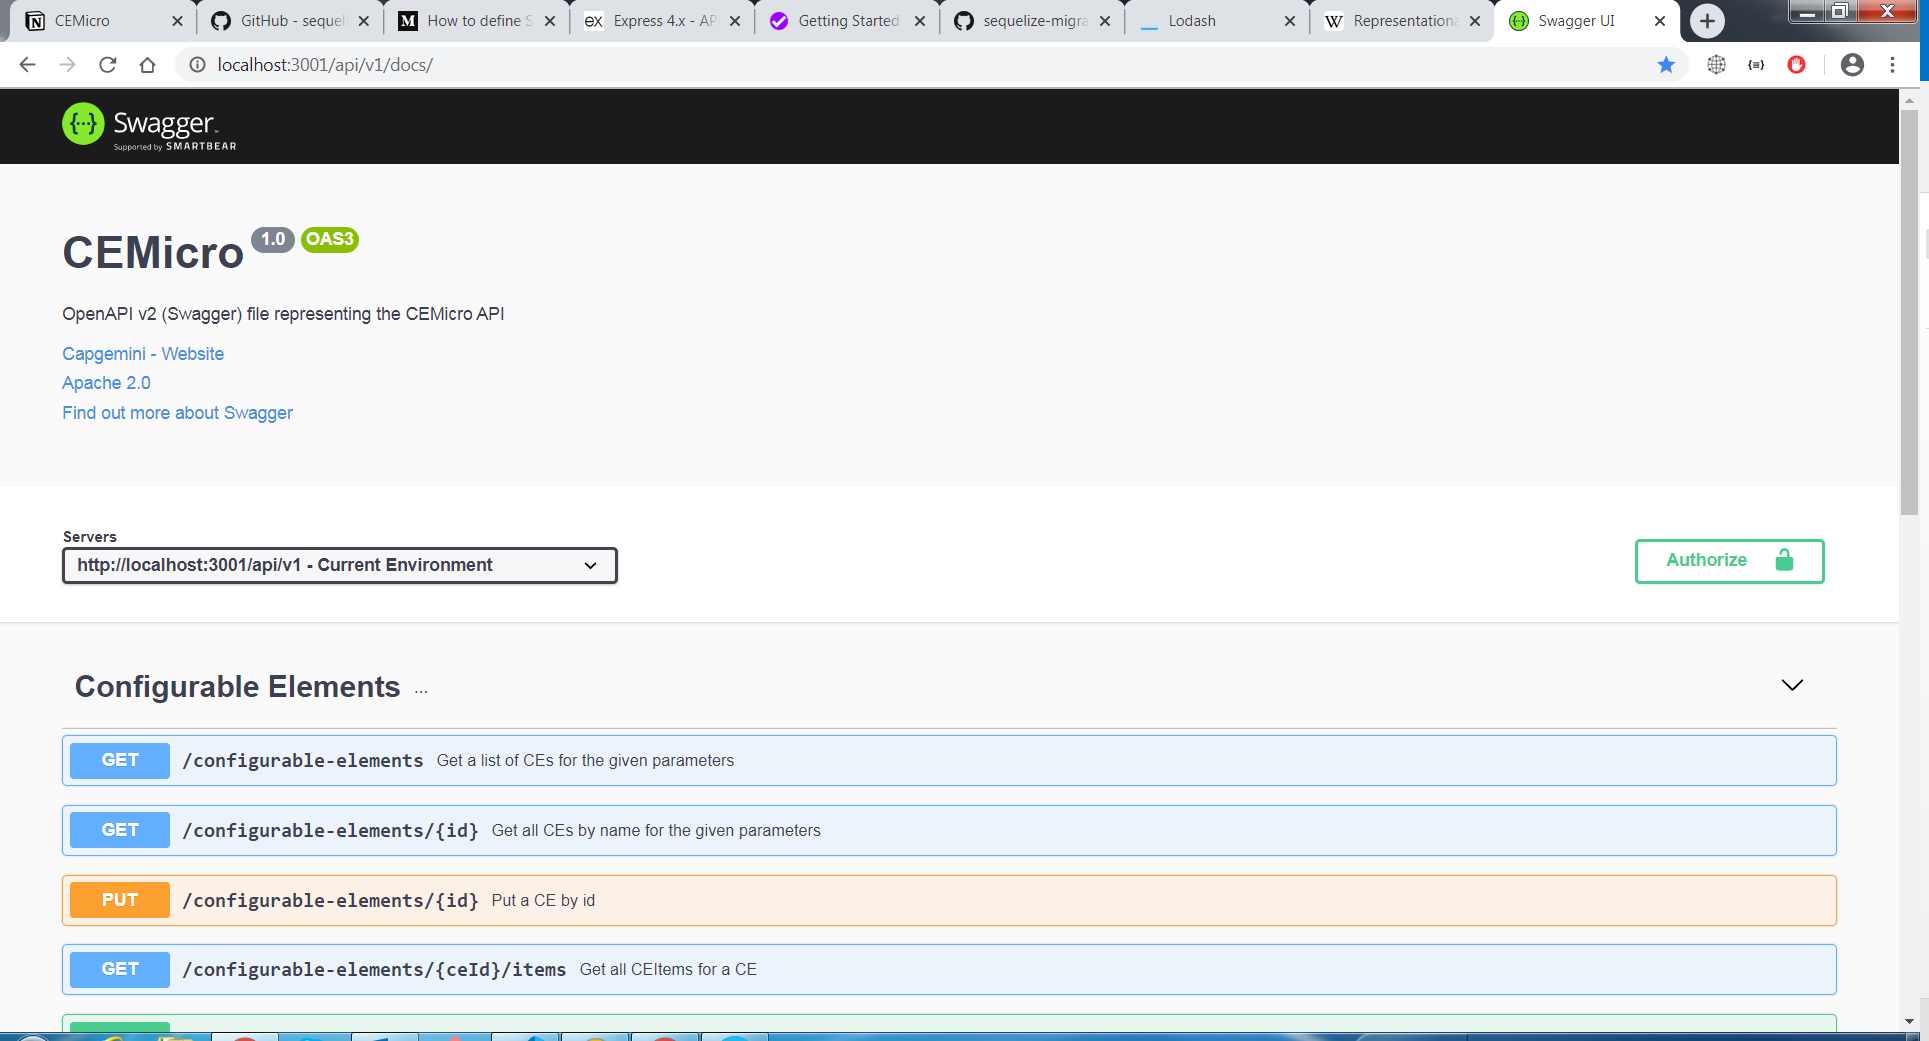
\includegraphics[width=0.8\linewidth]{assets/swagger-api-docs.png}
  \caption{Interactive API documentation with Swagger}
  \label{fig:api-docs}
\end{figure}


\section{Backend Framework with Express.js}

\begin{itemize}
  \item \todo{Tool: Nodemon}
  \item \todo{Tool: Express}
  \item \todo{Tool: Express Validator}
  \item \todo{MVC -> MVCS (Model View Controller Service)}
\end{itemize}


\section{Data persistance with PosgreSQL}

\begin{itemize}
  \item \todo{Sequelize https://github.com/sequelize/express-example}
  \item \todo{Discarded: Flyway-db, Umzug}
  \item \todo{Migrations: Sequelize}
\end{itemize}


\section{Frontend Framework with Vue.js}

\begin{itemize}
  \item \todo{To do ...}
\end{itemize}


\section{Virtualisation with Docker}

\begin{itemize}
 \item \todo{install packages, build, prune packages}
 \item \todo{...}
\end{itemize}


\section{Interfacing with the monolith development team}

\begin{itemize}
  \item \todo{Changes to Docify}
\end{itemize}


\section{Challanges during development}

\begin{itemize}
  \item \todo{Knowing how to set up the development environment}
  \item \todo{Understanding the task, see [CE Properties](https://www.notion.so/}CE-Properties-7bf08f28c69344c1957e7072c1101fd6)}
  \item \todo{Setting up git/bash on windows}
  \item \todo{File permissions for docker on windows ([https://medium.com/@akash1233/change-file-permissions-when-working-with-git-repos-on-windows-ea22e34d5cee](https://medium.com/@akash1233/change-file-permissions-when-working-with-git-repos-on-windows-ea22e34d5cee))}
\end{itemize}


\section{Documentation of CEMicro}

\begin{itemize}
  \item \todo{Providing a foundation for others to build on (Confluence, Readme, Thesis)}
\end{itemize}
